\newpage
\section*{はじめに}
バネで定在波を作って遊んでいるとき、振幅が最大のときのバネは振幅0のときに比べてどれぐらい伸びているのか気になったので調べてみた。波形はサインカーブであるから、サインの曲線に沿った長さを求めればよい。\par
ついでにカテナリー曲線についても調べた。これも日常よく見る曲線であり、知っておいて損はないかと思われる。

\chapter{サインカーブ}

\section{サインカーブの長さ}
\vspace{1zw}
\begin{center}
  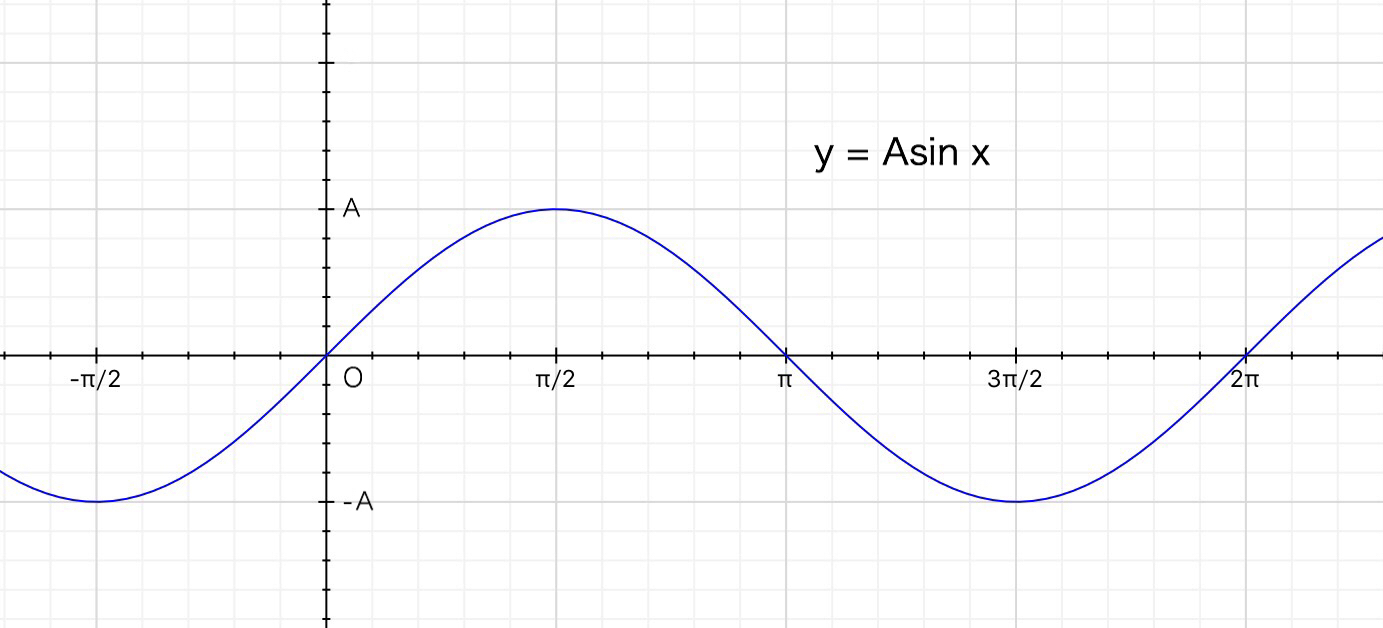
\includegraphics[width = 12cm]{nakayama/image/sine3.JPG}
\end{center}
\vspace{1zw}\par
$y = A \sin x$の曲線の長さを求めよう。求める長さを$L$とする。\par
\begin{wrapfigure}{r}{40mm}
\begin{center}
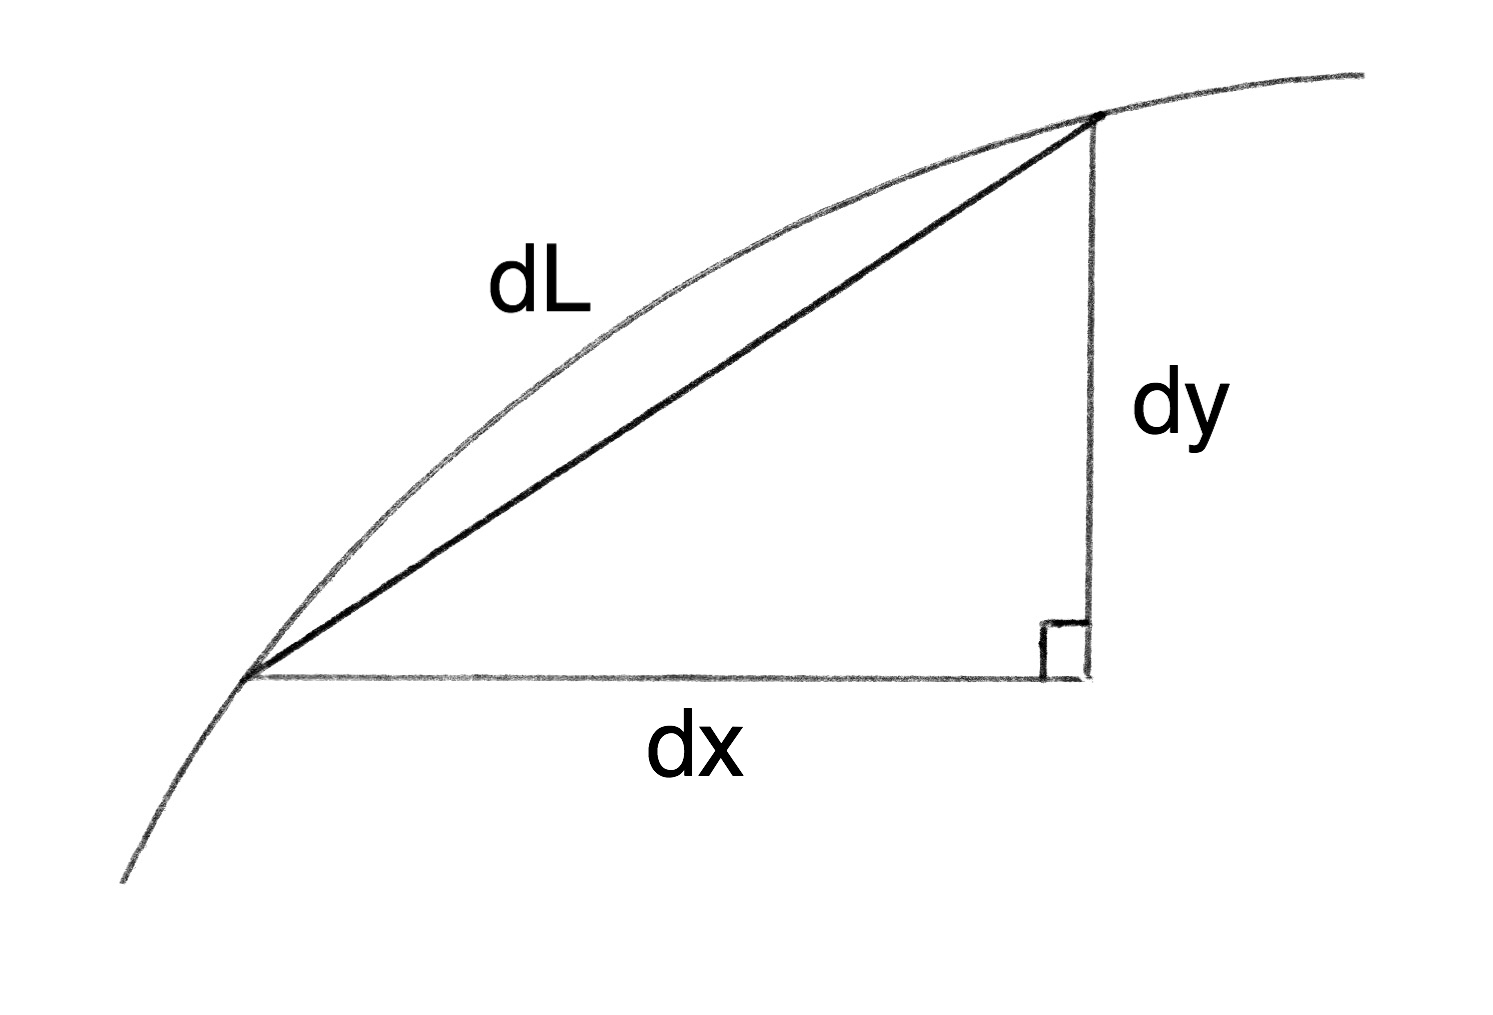
\includegraphics[width = 4cm]{nakayama/image/dL.jpg}
\end{center}
\end{wrapfigure}
微小長さ$dL$は三平方の定理より

\begin{eqnarray*}
dL & = & \sqrt{(dx)^2 + (dy)^2} \\
& = & \sqrt{1 + \left(\frac{dy}{dx}\right)^2}\,\,dx.
\end{eqnarray*}
\newline\par
よって
\begin{eqnarray*}
L & = & \int_{x_1}^{x_2} \sqrt{1 + \left(\frac{dy}{dx}\right)^2}\,\,dx \\
& = & \int_{x_1}^{x_2} \sqrt{1 + (A\cos x)^2}\,\,dx.
\end{eqnarray*}

あとはこれを計算するだけだが、どうにもこの積分は計算できそうにない。\par
もう少し変形してみると
\begin{eqnarray*}
L & = & \int_{x_1}^{x_2} \sqrt{1 + A^2(1 - \sin^2 x)}\,\,dx \\
& = & \int_{x_1}^{x_2} \sqrt{1 + A^2 - A^2\sin^2 x}\,\,dx \\
& = & \sqrt{A^2 + 1} \int_{x_1}^{x_2} \sqrt{1 - \frac{A^2}{A^2 + 1}\sin^2 x}\,\,dx
\end{eqnarray*}
となるが、この積分は第二種の楕円積分と呼ばれるもので、初等的には計算できないらしい。しかし、積分区間を$x =0〜\frac{\pi}{2}$とすることでなんとか級数の形にまでもっていくことができる。まずは次の2つの公式を用意しよう。


\section{準備}

\subsection{二項展開}

次の左辺は$|X| < 1$の条件のもとで
\begin{eqnarray*}
(1 - X)^a = \sum_{k=0}^\infty (-1)^k \binom{a}{k} X^k
\end{eqnarray*}
とテイラー展開できる\footnote{$a > 0$の場合、$X = \pm1$のときも収束する。}。\par
ここで$\binom ak$はコンビネーション$_aC_k$の$a$を実数の範囲にまで拡張したものであり
\begin{eqnarray*}
\binom ak = \frac{a(a-1)(a-2)\cdots(a-(k - 1))}{k!}
\end{eqnarray*}
と定義されている。ただし
$$
\binom a0 = 1
$$
とする。\par
上の式で$a = \frac{1}{2}$とすると
\begin{eqnarray*}
(1 - X)^\frac{1}{2} & = & \sum_{k=0}^\infty (-1)^k \binom{\frac{1}{2}}{k} X^k \\
& = & \binom{\frac{1}{2}}{0} + \sum_{k=1}^\infty (-1)^k \frac{\frac{1}{2} \left(\frac{1}{2} - 1 \right)\left(\frac{1}{2}-2\right) \cdots \left(\frac{1}{2} - (k - 1)\right)}{k!} X^k \\
& = & 1 + \sum_{k=1}^\infty (-1)^k \frac{\frac{1}{2} \left(-\frac{1}{2} \right)\left(-\frac{3}{2}\right) \cdots \left(-\frac{2k - 3}{2}\right)}{k!} X^k \\
& = & 1 + \sum_{k=1}^\infty (-1)^k\frac{(-1)^{k - 1}(2k - 3)\cdots3\cdot1}{2^k \cdot k!} X^k \\
& = & 1 - \sum_{k=1}^\infty \frac{(2k - 3)!!}{(2k)!!}  X^k
\end{eqnarray*}
を得る。ただし$(-1)!! = 1$と定義する。

\subsection{$\sin^Nx$の積分}

部分積分と漸化式を用いて$I_N = \int_0^{\frac{\pi}{2}}\sin^N x\,dx$を計算する。
\begin{eqnarray*}
I_N & = & \int_0^{\frac{\pi}{2}}\sin^N x\,dx \\
& = & \int_0^{\frac{\pi}{2}}\sin x \, \sin^{N - 1}x \,dx \\
& = & \int_0^{\frac{\pi}{2}}(-\cos x)^{'} \sin^{N - 1}x \,dx \\
& = & [-\cos x\,\sin^{N - 1}x]_0^\frac{\pi}{2} - \int_0^{\frac{\pi}{2}}(-\cos x)(N -1)\sin^{N - 2}x \cos x\,dx \\
& = & 0 + (N - 1)\int_0^{\frac{\pi}{2}}\cos^2 x\,\sin^{N - 2}x\,dx \\
& = & (N - 1)\int_0^{\frac{\pi}{2}}(1 - \sin^2x)\,\sin^{N - 2}x\,dx \\
& = & (N - 1)\int_0^{\frac{\pi}{2}}(\sin^{N - 2}x - \sin^Nx)\,dx \\
& = & (N - 1)\,I_{N - 2} - (N - 1)\,I_N.
\end{eqnarray*}

よって、以下の漸化式が成立する。
\begin{eqnarray*}
I_N = \frac{N - 1}{N}\,I_{N - 2}.
\end{eqnarray*}

$I_0=\frac{\pi}{2}$であるから、Nが偶数のとき
\begin{eqnarray*}
I_N & = & \frac{N - 1}{N}\,I_{N - 2} \\
& = & \frac{N - 1}{N}\frac{N - 3}{N - 2}\,I_{N - 4} \\
& = & \cdots \quad=\,\,\, \frac{(N - 1)!!}{N!!}\,I_0 \\
& = & \frac{(N - 1)!!}{N!!}\frac{\pi}{2}
\end{eqnarray*}
となる。


\section{サインカーブの長さ 続き}

\subsection{楽しい計算}

準備が整った。これでようやく積分の続きが計算できる。ただし積分区間は$x=0〜\frac{\pi}{2}$とする。
\begin{eqnarray*}
L & = & \sqrt{A^2 + 1} \int_0^\frac{\pi}{2} \sqrt{1 - \frac{A^2}{A^2 + 1}\sin^2 x}\,\,dx \\
& = & \sqrt{A^2 + 1} \int_0^\frac{\pi}{2} \left(1 - \frac{A^2}{A^2 + 1}\sin^2 x \right)^\frac{1}{2}\,dx
\end{eqnarray*}
$|\frac{A^2}{A^2 + 1}\sin^2 x| \leq 1$であるから、2.2.1より
\begin{eqnarray*}
\qquad\qquad\qquad\quad & = & \sqrt{A^2 + 1} \int_0^\frac{\pi}{2}\left(1 - \sum^{\infty}_{k = 1}\frac{(2k - 3)!!}{(2k)!!}\left(\frac{A^2}{A^2 + 1}\sin^2 x\right)^k\,\right)dx \\
& = & \sqrt{A^2 + 1} \left(\int_0^\frac{\pi}{2}dx - \sum^{\infty}_{k = 1}\frac{(2k - 3)!!}{(2k)!!}\left(\frac{A^2}{A^2 + 1}\right)^k \int_0^\frac{\pi}{2}\sin^{2k}x\,dx \right)
\end{eqnarray*}
2.2.2より
\begin{eqnarray*}
\qquad\qquad\qquad\quad & = & \sqrt{A^2 + 1} \left(\frac{\pi}{2} - \sum^{\infty}_{k = 1}\frac{(2k - 3)!!}{(2k)!!}\left(\frac{A^2}{A^2 + 1}\right)^k\frac{(2k - 1)!!}{(2k)!!}\frac{\pi}{2} \right)\\
& = & \frac{\pi}{2}\sqrt{A^2 + 1} \left(1 - \sum^{\infty}_{k = 1}\frac{(2k - 1)!!}{(2k)!!(2k - 1)}\left(\frac{A^2}{A^2 + 1}\right)^k\frac{(2k - 1)!!}{(2k)!!}\right) \\
& = & \frac{\pi}{2}\sqrt{A^2 + 1} \left(1 + \sum^{\infty}_{k = 1}\left(\frac{(2k - 1)!!}{(2k)!!}\right)^2 \left(\frac{A^2}{A^2 + 1}\right)^k\frac{1}{1 - 2k} \right) \\
& = & \frac{\pi}{2}\sqrt{A^2 + 1}\,\sum^{\infty}_{k = 0}\left(\frac{(2k - 1)!!}{(2k)!!}\right)^2 \left(\frac{A^2}{A^2 + 1}\right)^k\frac{1}{1 - 2k}.
\end{eqnarray*}

これで$L$を級数で表すことができた。

\subsection{具体的な数値}

$\displaystyle L = \frac{\pi}{2}\sqrt{A^2 + 1}\,\sum^{n}_{k = 0}\left(\frac{(2k - 1)!!}{(2k)!!}\right)^2\left(\frac{A^2}{A^2 + 1}\right)^k\frac{1}{1 - 2k}$で近似を計算した。表の値は小数点以下7桁目を四捨五入している。参考までに、$\frac{\pi}{2}=1.570596...$ である。\\

\begin{table}[ht]
\begin{center}
\begin{tabular}{cc}

\begin{minipage}{0.5\hsize}
\begin{center}
A = 1 \\
\begin{tabular}{c|c} \hline
n & L \\ \hline
1 & 1.943761 \\
2 & 1.917729 \\
3 & 1.912305 \\
4 & 1.910822 \\
5 & 1.910355 \\
6 & 1.910195 \\
7 & 1.910136 \\
8 & 1.910114 \\
9 & 1.910105 \\
10 & 1.910101 \\ \hline
正確な値 & 1.9100988945... \\ \hline
\end{tabular}
\end{center}
\end{minipage}

\begin{minipage}{0.5\hsize}
\begin{center}
A = 2 \\
\begin{tabular}{c|c} \hline
n & L \\ \hline
1 & 2.809926 \\
2 & 2.704554 \\
3 & 2.669430 \\
4 & 2.654063 \\
5 & 2.646318 \\
6 & 2.642058 \\
7 & 2.639572 \\
8 & 2.638057 \\
9 & 2.637103 \\
10 & 2.636487 \\ \hline
正確な値 & 2.6351835815... \\ \hline
\end{tabular}
\end{center}
\end{minipage}

\end{tabular}
\end{center}
\end{table}

\begin{table}[htb]
\begin{center}
\begin{tabular}{cc}

\begin{minipage}{0.5\hsize}
\begin{center}
A = 0.3 \\
\begin{tabular}{c|c} \hline
n & L \\ \hline
1 & 1.606107 \\
2 & 1.605583 \\
3 & 1.605565 \\
4 & 1.605564 \\
5 & 1.605564 \\ \hline
正確な値 & 1.6055641558... \\ \hline
\end{tabular}
\end{center}
\end{minipage}

\begin{minipage}{0.5\hsize}
\begin{center}
A = 0.5 \\
\begin{tabular}{c|c} \hline
n & L \\ \hline
1 & 1.668393 \\
2 & 1.665101 \\
3 & 1.664826 \\
4 & 1.664796 \\
5 & 1.664792 \\ \hline
正確な値 & 1.664791805... \\ \hline

\end{tabular}
\end{center}
\end{minipage}

\end{tabular}
\end{center}
\end{table}

\clearpage
\section{(参考)楕円積分}
$$
E(x, m) = \int_0^x \sqrt{1 - m\sin^2 \theta}\,\,d\theta
$$
を第二種楕円積分という。また、$x = \frac{\pi}{2}$としたものを第二種完全楕円積分という。
$$
E(m) = E\left(\frac{\pi}{2}, m\right) = \int_0^\frac{\pi}{2} \sqrt{1 - m\sin^2 \theta}\,\,d\theta.
$$ \par
これを使うと、先ほど求めた$y = A\sin x$の曲線の長さ$L$は
$$
L = \sqrt{1 + A^2}\,\,E\left(\frac{A^2}{1 + A^2}\right)
$$
と書くことができる。\par
楕円積分には他にも第一種、第三種がある。振り子の周期を計算するときには第一種の楕円積分が出てくる。暇な人は計算してみるとよい。

\chapter{カテナリー曲線}
\section{カテナリー曲線とは}
ロープや電線などの両端を持って垂らしたときにできる曲線のことをカテナリー曲線または懸垂曲線という。\\
\begin{center}
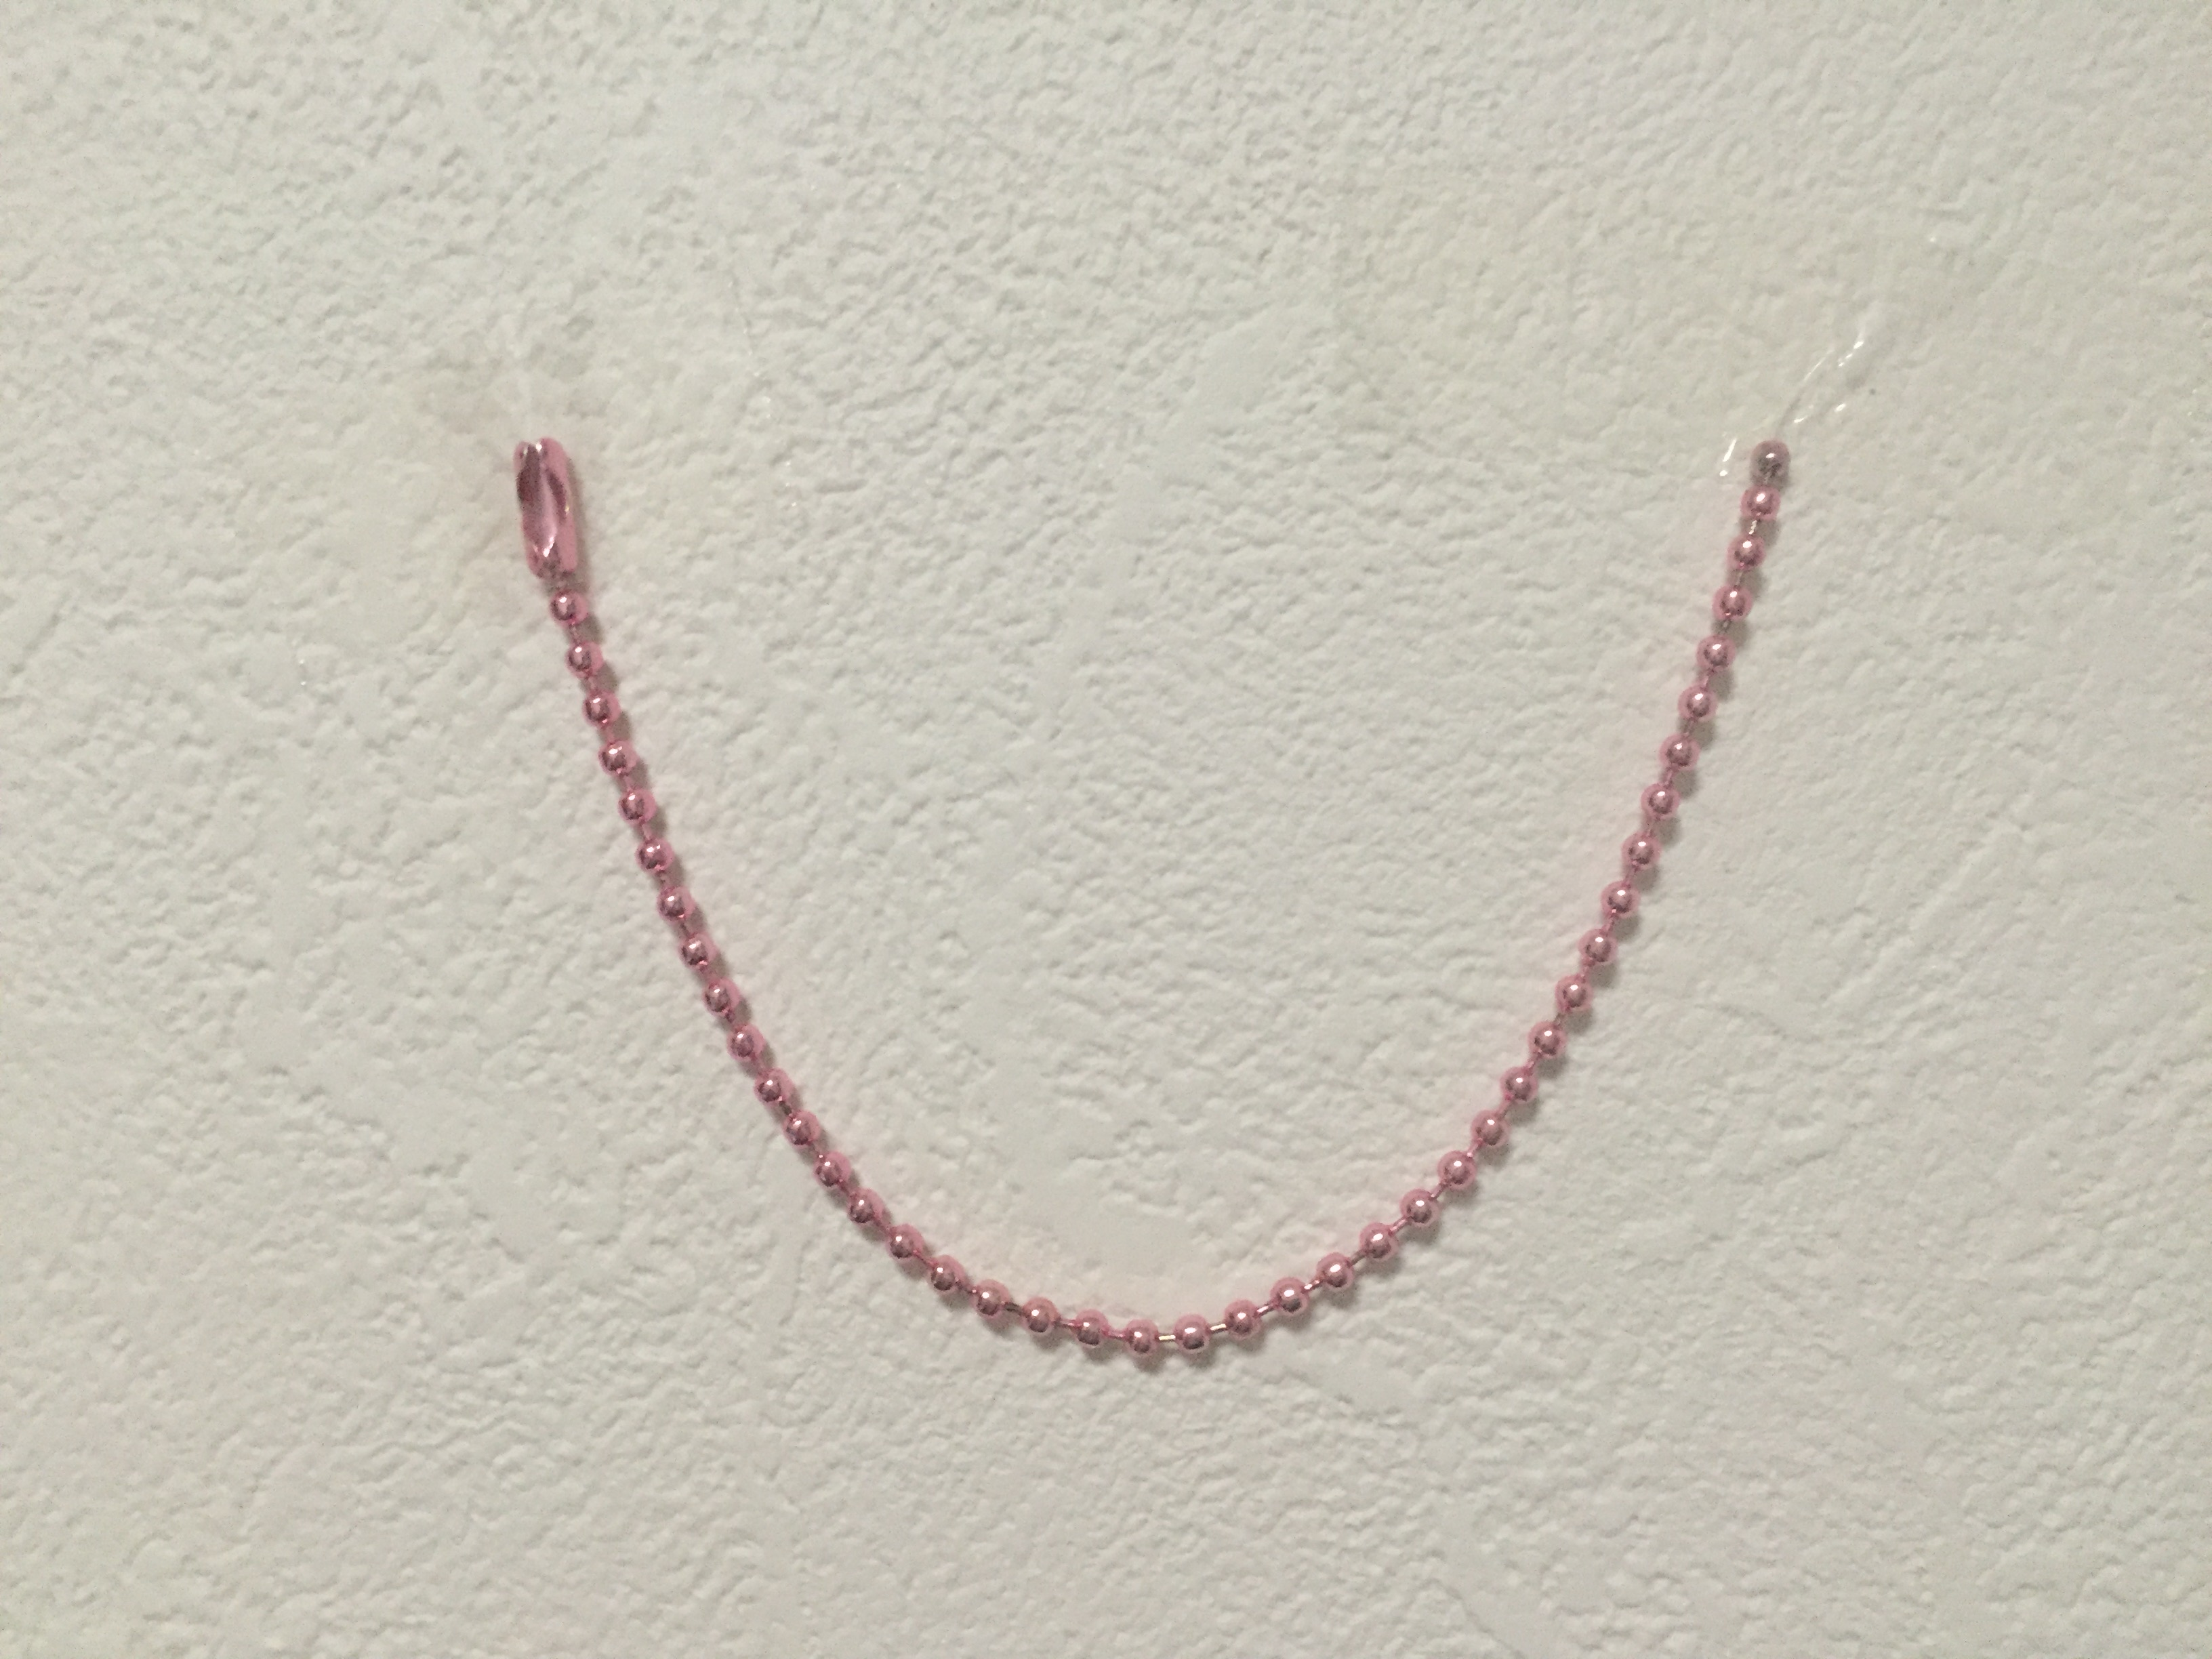
\includegraphics[width = 5cm]{nakayama/image/chen.JPG}
\quad
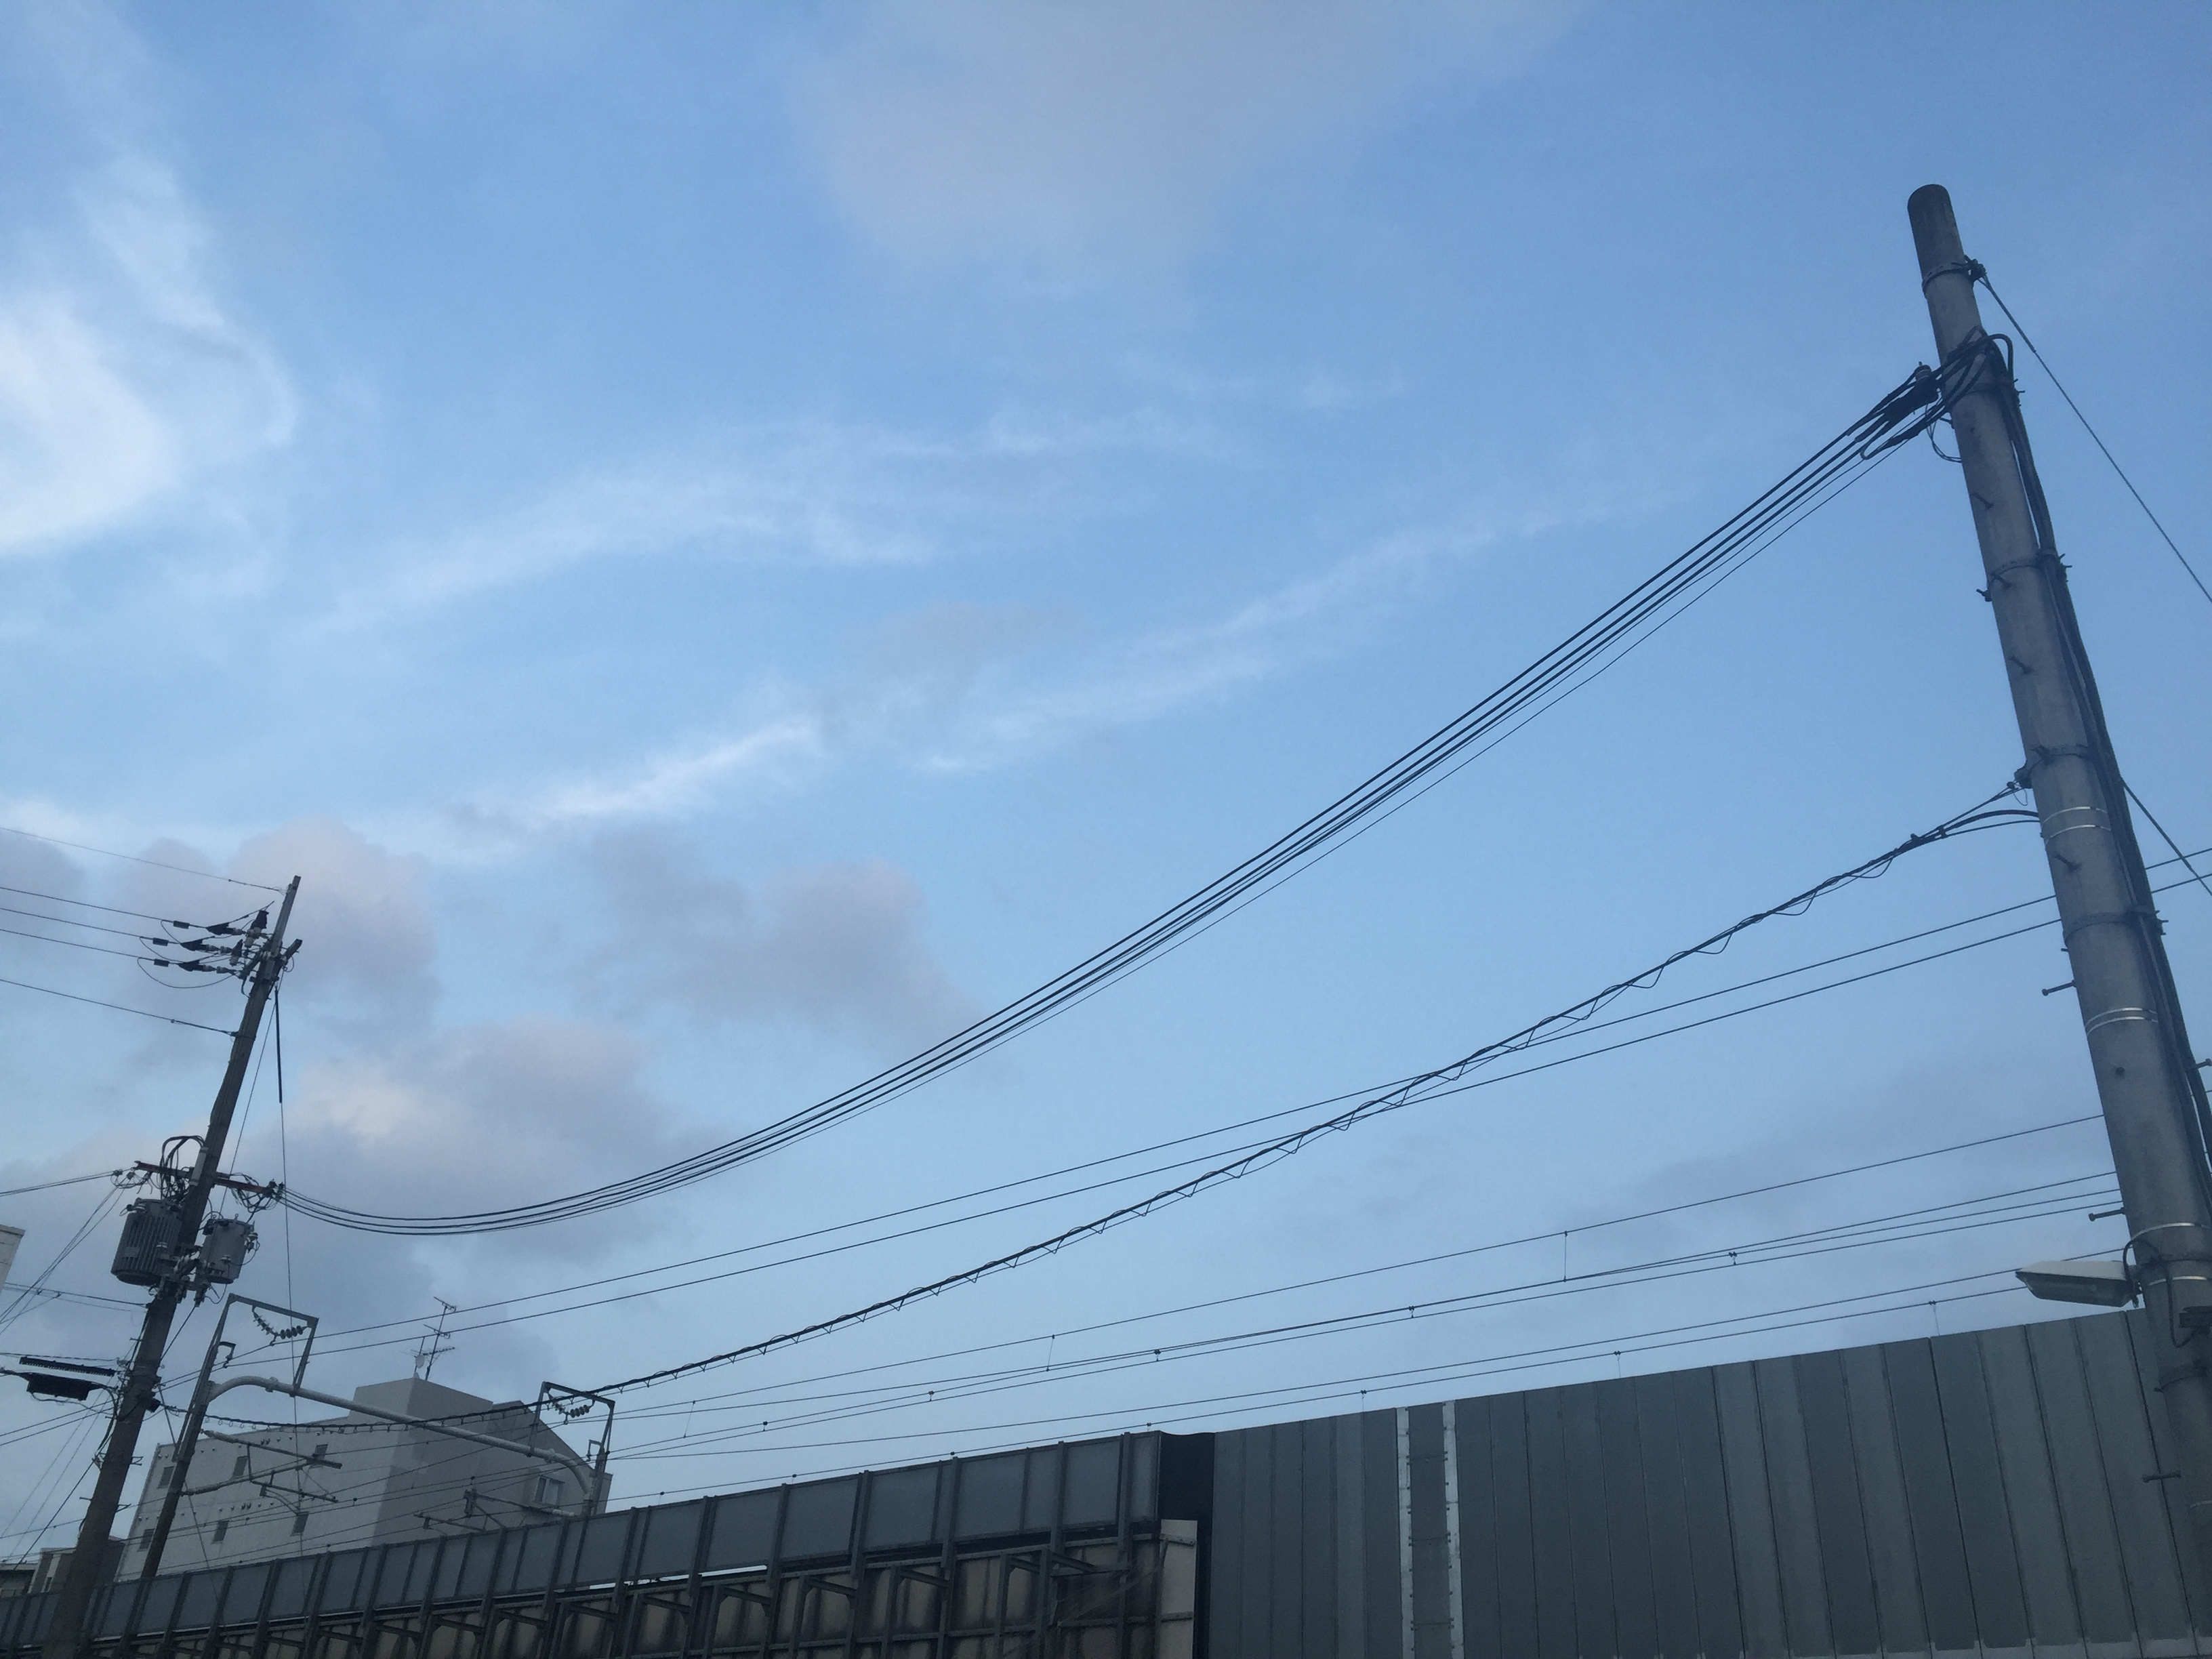
\includegraphics[width = 5cm]{nakayama/image/densen.JPG}
\end{center}

\section{曲線の方程式}
まずはカテナリー曲線の方程式を求める。曲線は、頂点における法線を軸として線対称であり、一様な質量の線密度を持つものと仮定する。

カテナリー上で頂点($x$座標を$0$とする)からの弧長が$s$であるような点$(x, y)$において、その接線が$x$軸の正の向きと成す角を$\theta$と置くとき、頂点から点$(x, y)$までの弧に掛かる力の釣り合いを考える。重力加速度を$g$、曲線の線密度を$w$とすれば、点$(x, y)$における張力$T$の鉛直成分 $T\sin{\theta}$は、頂点から点$(x, y)$までの弧にかかる重力$wgs$と釣り合う。また、頂点における張力は水平成分のみであり、この大きさを$k$とすると、点$(x,y)$における張力の水平成分$T\cos{\theta}$と釣り合う。
\begin{center}
  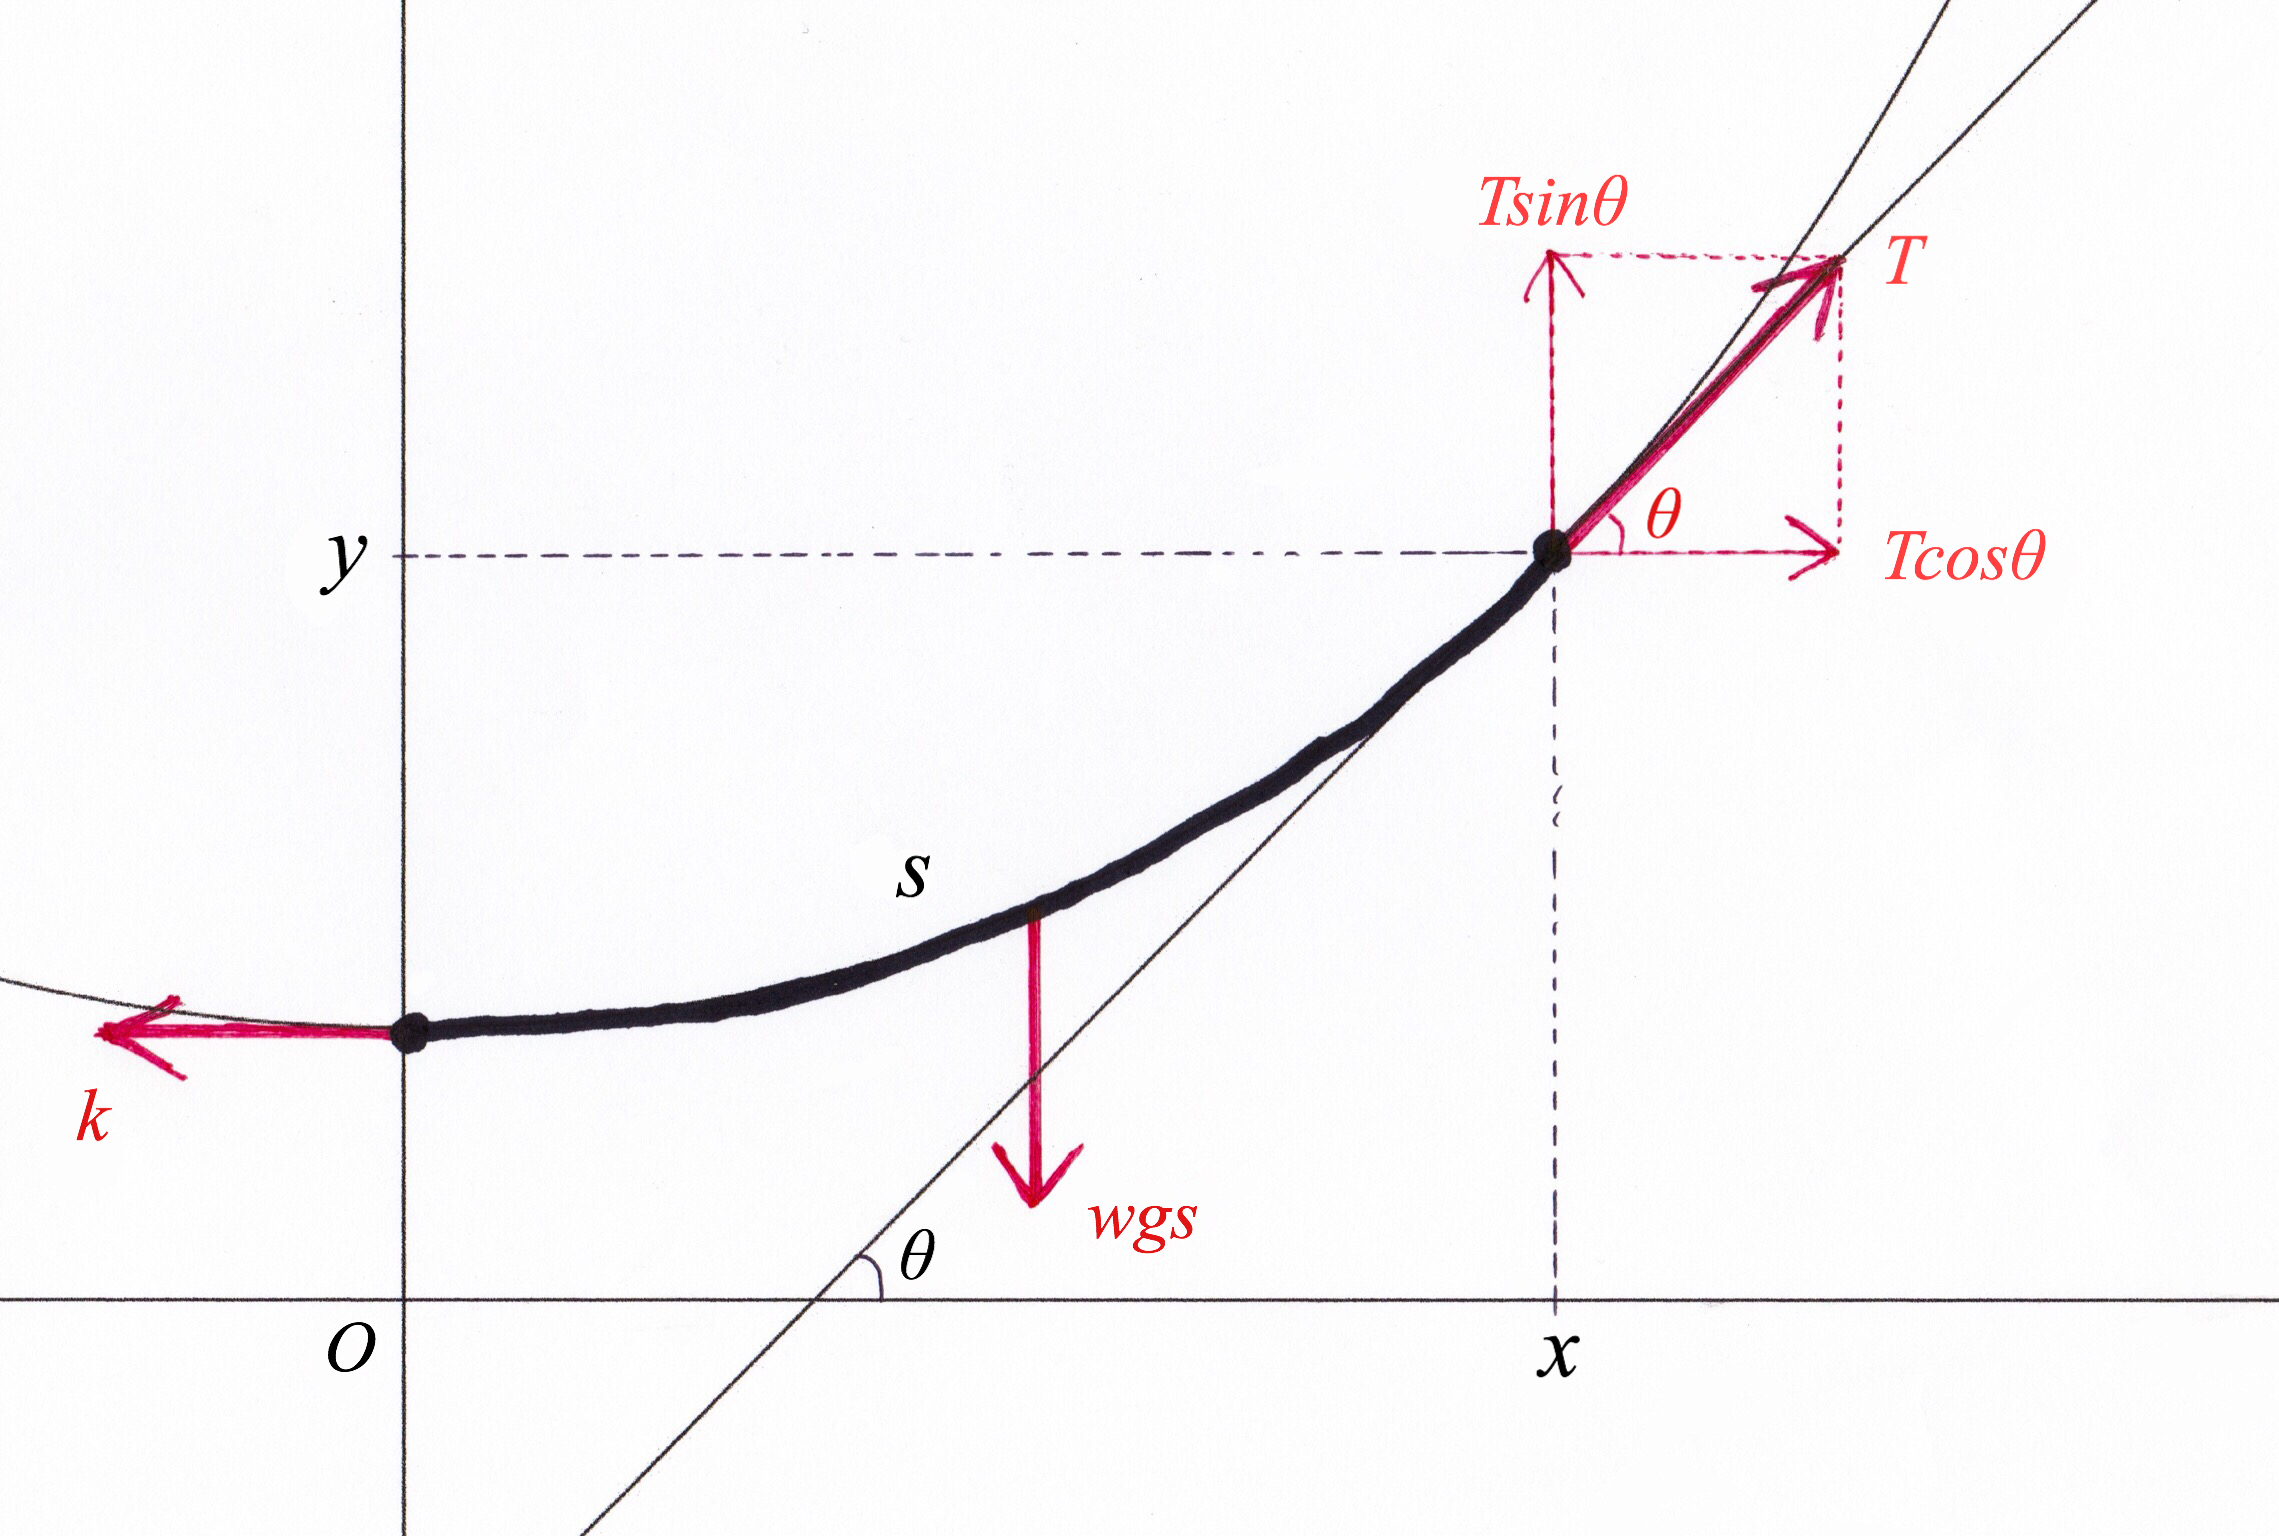
\includegraphics[width = 8cm]{nakayama/image/catenary2.JPG}
\end{center}
\vspace{-0.5zw}
\begin{displaymath}
\left\{
\begin{array}{l}
T\sin{\theta} = wgs \\
T\cos{\theta} = k \\
\tan{\theta} = \dfrac{dy}{dx}
\end{array}
\right.
\end{displaymath}
という条件が得られるので、これを解く。\\

3式から
\begin{eqnarray*}
\tan{\theta} = \frac{dy}{dx} = \frac{wgs}{k}.
\end{eqnarray*}

$\frac{k}{wg} = a$とおいて
\begin{eqnarray*}
\frac{dy}{dx} & = & \frac{s}{a}.
\end{eqnarray*}

よって
\begin{eqnarray*}
\frac{ds}{dx} & = & \frac{\sqrt{dx^2 + dy^2}}{dx} \\
& = & \sqrt{1 + \left(\frac{dy}{dx} \right)^2} \\
& = & \sqrt{1 + \left(\frac{s}{a} \right)^2} \\
& = & \frac{\sqrt{s^2 + a^2}}{a} \\
\frac{ds}{\sqrt{s^2 + a^2}} & = & \frac{dx}{a}
\end{eqnarray*}
両辺積分して
\begin{eqnarray*}
(右辺) & = & \int \frac{dx}{a}\qquad\quad \\
& = & \frac{x}{a} + C_1.
\end{eqnarray*}

\begin{eqnarray*}
(左辺) & = & \int \frac{ds}{\sqrt{s^2 + a^2}}
\end{eqnarray*}
$s = a\sinh t$とおくと、$\frac{ds}{dt} = a\cosh t$であるから
\begin{eqnarray*}
\qquad\qquad\qquad\quad & = & \int \frac{a\cosh t}{\sqrt{(a\sinh t)^2 + a^2}}\,\,dt \\
& = & \int \frac{\cosh t}{\sqrt{\sinh^2 t + 1}}\,\,dt
\end{eqnarray*}
$1 + \sinh^2 t = \cosh^2 t$より
\begin{eqnarray*}
\qquad\qquad & = & \int \frac{\cosh t}{\sqrt{\cosh^2 t}}\,\,dt \\
& = & \int dt \\
& = & t + C_2 \\
& = & \sinh^{-1}\frac{s}{a} +C_2.
\end{eqnarray*}

よって
\begin{eqnarray*}
\sinh^{-1}\frac{s}{a} & = & \frac{x}{a} + C_3.
\end{eqnarray*}

$x = 0$のとき$s = 0$であるから$C_3 = 0$. \\

よって
\begin{eqnarray*}
\sinh^{-1}\frac{s}{a} & = & \frac{x}{a} \\
s & = & a\sinh\frac{x}{a}.
\end{eqnarray*}

また
\begin{eqnarray*}
\frac{ds}{dy} & = & \frac{\sqrt{dx^2 + dy^2}}{dy} \\
& = & \sqrt{\left(\frac{dx}{dy}\right)^2 + 1} \\
& = & \sqrt{\left(\frac{a}{s}\right)^2 + 1} \\
& = & \frac{\sqrt{s^2 + a^2}}{s} \\
\frac{s}{\sqrt{s^2 + a^2}}\,\,ds & = & dy
\end{eqnarray*}
両辺積分して
\begin{eqnarray*}
\int \frac{s}{\sqrt{s^2 + a^2}}\,\,ds & = & \int dy\qquad\qquad\quad \\
\sqrt{s^2 + a^2} & = & y + C_4.
\end{eqnarray*}

$s = 0$のとき$y = a$とすると$C_4 = 0$.

よって
\begin{eqnarray*}
\sqrt{s^2 + a^2} & = & y.\qquad\quad\quad
\end{eqnarray*}

以上の2式から$s$を消去して
\begin{eqnarray*}
y & = & \sqrt{\left(a\sinh \frac{x}{a}\right)^2 + a^2} \\
& = & a\sqrt{1 + \sinh^2 \frac{x}{a}} \\
& = & a\cosh{\frac{x}{a}}.
\end{eqnarray*}
となる。\par
係数は$a = \frac{k}{wg}$であるので、横の引っ張りが弱い、または重力が大きいとよく弛むことがわかる。\\\\

\begin{center}
  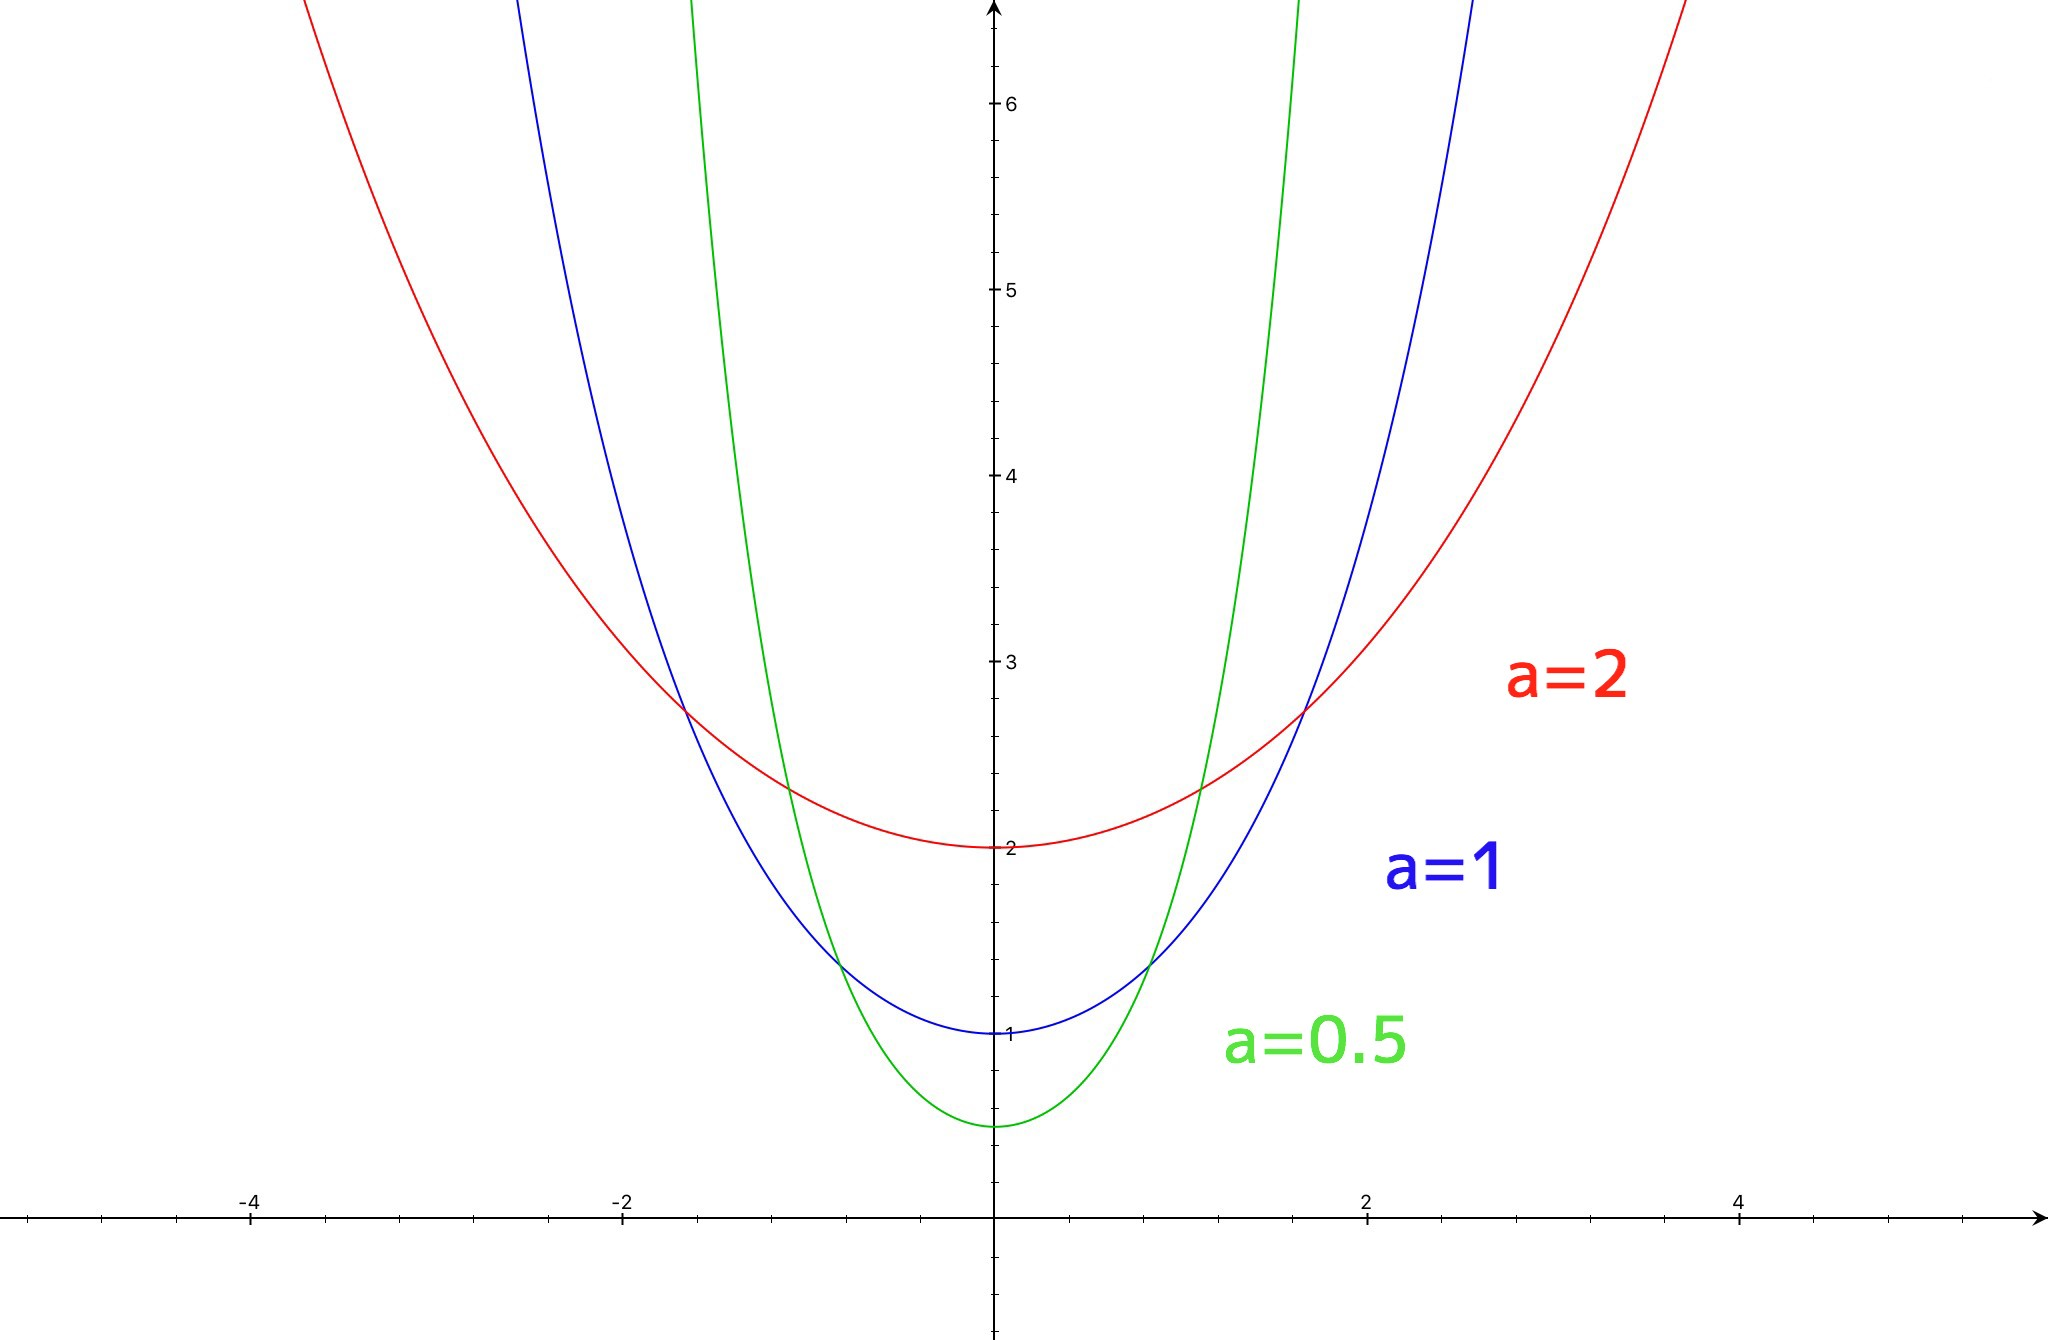
\includegraphics[width = 11cm]{nakayama/image/catenary1.JPG}
\end{center}


\newpage
\section{曲線の長さ}
\subsection{積分計算}

カテナリー曲線は$y = a\cosh{\frac{x}{a}}$で表せることがわかった。頂点の座標は$(0,a)$である。

それでは曲線の長さ$L$を求めよう。径間距離(ひもを支える2点間の距離)を$D$とすると
\begin{eqnarray*}
L & = & \int_{-D}^D ds \\
& = & 2 \int_0^\frac{D}{2} ds \\
& = & 2 \int_0^\frac{D}{2} \sqrt{dx^2 + dy^2} \\
& = & 2 \int_0^\frac{D}{2} \sqrt{1 + \left(\frac{dy}{dx}\right)^2}\,\,dx \\
& = & 2 \int_0^\frac{D}{2} \sqrt{1 + \sinh^2\frac{x}{a}}\,\,dx \\
& = & 2 \int_0^\frac{D}{2} \cosh \frac{x}{a}\,\,dx \\
& = & 2 \left[a\sinh \frac{x}{a}\right]_0^\frac{D}{2} \\
& = & 2a\sinh\frac{D}{2a} \\
& = & 2a\cdot\frac{\, e^{\frac{D}{2a}} - e^{-\frac{D}{2a}}}{2}
\end{eqnarray*}\par
指数関数をテイラー展開して
\begin{eqnarray*}
\qquad\qquad\qquad\quad & = & a\left(\sum_{k = 0}^\infty \frac{1}{k!}\left(\frac{D}{2a}\right)^k - \sum_{k = 0}^\infty \frac{1}{k!}\left(-\frac{D}{2a}\right)^k\right)
\end{eqnarray*}\par
$k = 2j + 1$(奇数)の項だけ残って
\begin{eqnarray*}
\qquad & = & 2a\sum_{j = 0}^\infty \frac{1}{(2j + 1)!}\left(\frac{D}{2a}\right)^{2j + 1}
\end{eqnarray*}\par
$j$を改めて$k$とおいて整理すると
\begin{eqnarray*}
& = & \sum_{k = 0}^\infty \frac{D^{2k + 1}}{(2a)^{2k}(2k + 1)!}. \quad
\end{eqnarray*}

これで$L$を級数で表すことができた。

\subsection{具体的な数値}
$\displaystyle L = \sum_{k = 0}^n \frac{D^{2k + 1}}{(2a)^{2k}(2k + 1)!}$で近似を計算した。表の値は小数点以下7桁目を四捨五入している。\\\par
$D = 2$のとき
\begin{table}[htb]
\begin{center}
\begin{tabular}{cc}

\begin{minipage}{0.5\hsize}
\begin{center}
a = 0.5 \\
\begin{tabular}{c|c} \hline
n & L \\ \hline
1 & 3.333333 \\
2 & 3.600000 \\
3 & 3.625397 \\
4 & 3.626808 \\
5 & 3.626859 \\ \hline
正確な値 & 3.62686040784... \\ \hline
\end{tabular}
\end{center}
\end{minipage}

\end{tabular}
\end{center}
\end{table}


\begin{table}[htb]
\begin{center}
\begin{tabular}{cc}

\begin{minipage}{0.5\hsize}
\begin{center}
a = 1 \\
\begin{tabular}{c|c} \hline
n & L \\ \hline
1 & 2.333333 \\
2 & 2.350000 \\
3 & 2.350397 \\
4 & 2.350402 \\ \hline
正確な値 & 2.35040238728... \\ \hline
\end{tabular}
\end{center}
\end{minipage}

\begin{minipage}{0.5\hsize}
\begin{center}
a = 2 \\
\begin{tabular}{c|c} \hline
n & L \\ \hline
1 & 2.083333 \\
2 & 2.084375 \\
3 & 2.084381 \\
4 & 2.084381 \\ \hline
正確な値 & 2.08438122197... \\ \hline
\end{tabular}
\end{center}
\end{minipage}

\end{tabular}
\end{center}
\end{table}

\clearpage
$D = 5$のとき

\begin{table}[htb]
\begin{center}
\begin{tabular}{cc}

\begin{minipage}{0.5\hsize}
\begin{center}
a = 0.5 \\
\begin{tabular}{c|c} \hline
n & L \\ \hline
1 & 25.833333 \\
2 & 51.875000 \\
3 & 67.375992 \\
4 & 72.758281 \\
5 & 73.981528 \\
6 & 74.177562 \\ \hline
正確な値 & 74.203210577788... \\ \hline
\end{tabular}
\end{center}
\end{minipage}

\end{tabular}
\end{center}
\end{table}

%
\begin{table}[htb]
\begin{center}
\begin{tabular}{cc}
%
\begin{minipage}{0.5\hsize}
\begin{center}
a = 1 \\
\begin{tabular}{c|c} \hline
n & L \\ \hline
1 & 10.208333 \\
2 & 11.835938 \\
3 & 12.078141 \\
4 & 12.099165 \\
5 & 12.100360 \\ \hline
正確な値 & 12.1004089620... \\ \hline
\end{tabular}
\end{center}
\end{minipage}
%
\begin{minipage}{0.5\hsize}
\begin{center}
a = 2 \\
\begin{tabular}{c|c} \hline
n & L \\ \hline
1 & 6.302083 \\
2 & 6.403809 \\
3 & 6.407593 \\
4 & 6.407675 \\
5 & 6.407676 \\ \hline
正確な値 & 6.40767632120... \\ \hline
\end{tabular}
\end{center}
\end{minipage}
%
\end{tabular}
\end{center}
\end{table}
%
\section*{参考文献}
\begin{enumerate}
  \item	吉田武,『新装版 オイラーの贈物』(東海大出版部,2015)
  \item \url{http://mathtrain.jp/int_sinnx},『sinのn乗,cosのn乗の積分公式』
  \item \url{https://ja.wikipedia.org/wiki/楕円積分}
  \item \url{https://ja.wikipedia.org/wiki/カテナリー曲線}
  \item \url{http://mathtrain.jp/catenary},『懸垂線の2通りの導出』
\end{enumerate}
